\documentclass[border=3pt]{standalone}
% Preâmbulo compartilhado pelos diagramas TikZ da aula
\usepackage[T1]{fontenc}
\usepackage[utf8]{inputenc}
\usepackage{lmodern}
\usepackage{amsmath}
\usepackage{xcolor}
\usepackage{tikz}
\usetikzlibrary{arrows.meta,angles,quotes,decorations.pathmorphing,calc,
                positioning,shapes.geometric,backgrounds,fit}

% Paleta (mesma dos SVGs originais)
\definecolor{dblue}{HTML}{2A5B8C}
\definecolor{dorange}{HTML}{B3541E}
\definecolor{dgreen}{HTML}{4A7C59}
\definecolor{dred}{HTML}{9C4B4B}
\definecolor{dcream}{HTML}{F4F1EA}
\definecolor{dshade}{HTML}{DDD7C9}

% Estilos comuns (prefixo d... para não colidir com chaves internas do pgf)
\tikzset{
  >={Stealth[length=2mm]},
  dguide/.style={gray!55, dashed, line width=0.4pt},
  daxis/.style={gray!60, line width=0.7pt, ->},
  dbody/.style={fill=black!3, draw=black!80, line width=1pt},
  dacc/.style={draw=dblue, line width=1pt},
  dlbl/.style={black!55, font=\small},
  dsub/.style={black!45, font=\footnotesize},
  dstate/.style={circle, draw=black!80, fill=dcream, line width=1pt,
                 minimum size=17mm, font=\large, inner sep=1pt},
  dobs/.style={circle, draw=black!80, fill=dshade, line width=1pt,
               minimum size=14mm, font=\large, inner sep=1pt},
  dbox/.style={rounded corners=2pt, draw=black!80, fill=dcream, line width=1pt,
               align=center, inner sep=6pt},
  dtrans/.style={->, dblue, line width=1pt},
  dmeas/.style={->, dorange, line width=1pt},
}

\begin{document}
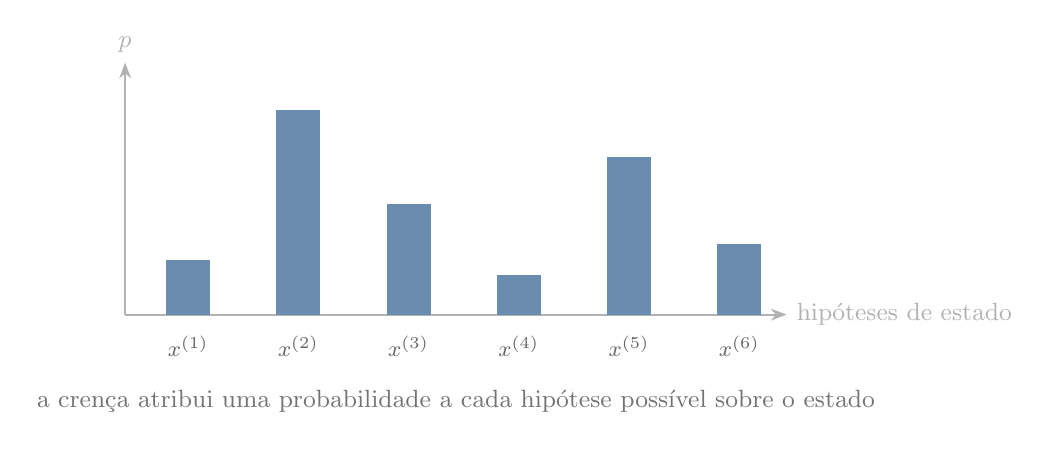
\begin{tikzpicture}[x=1cm,y=1cm]

  \draw[daxis] (0,0) -- (8.4,0) node[right, font=\small] {hipóteses de estado};
  \draw[daxis] (0,0) -- (0,3.2) node[above, font=\small] {$p$};

  \foreach \x/\h/\lab in {0.8/0.7/{$x^{(1)}$}, 2.2/2.6/{$x^{(2)}$}, 3.6/1.4/{$x^{(3)}$},
                         5.0/0.5/{$x^{(4)}$}, 6.4/2.0/{$x^{(5)}$}, 7.8/0.9/{$x^{(6)}$}}
  {
    \fill[dblue!70] (\x-0.28,0) rectangle (\x+0.28,\h);
    \node[black!60, font=\footnotesize] at (\x,-0.4) {\lab};
  }

  \node[dlbl] at (4.2,-1.1)
    {a crença atribui uma probabilidade a cada hipótese possível sobre o estado};

\end{tikzpicture}
\end{document}
